% Options for packages loaded elsewhere
\PassOptionsToPackage{unicode}{hyperref}
\PassOptionsToPackage{hyphens}{url}
%
\documentclass[
]{article}
\usepackage{amsmath,amssymb}
\usepackage{lmodern}
\usepackage{ifxetex,ifluatex}
\ifnum 0\ifxetex 1\fi\ifluatex 1\fi=0 % if pdftex
  \usepackage[T1]{fontenc}
  \usepackage[utf8]{inputenc}
  \usepackage{textcomp} % provide euro and other symbols
\else % if luatex or xetex
  \usepackage{unicode-math}
  \defaultfontfeatures{Scale=MatchLowercase}
  \defaultfontfeatures[\rmfamily]{Ligatures=TeX,Scale=1}
\fi
% Use upquote if available, for straight quotes in verbatim environments
\IfFileExists{upquote.sty}{\usepackage{upquote}}{}
\IfFileExists{microtype.sty}{% use microtype if available
  \usepackage[]{microtype}
  \UseMicrotypeSet[protrusion]{basicmath} % disable protrusion for tt fonts
}{}
\makeatletter
\@ifundefined{KOMAClassName}{% if non-KOMA class
  \IfFileExists{parskip.sty}{%
    \usepackage{parskip}
  }{% else
    \setlength{\parindent}{0pt}
    \setlength{\parskip}{6pt plus 2pt minus 1pt}}
}{% if KOMA class
  \KOMAoptions{parskip=half}}
\makeatother
\usepackage{xcolor}
\IfFileExists{xurl.sty}{\usepackage{xurl}}{} % add URL line breaks if available
\IfFileExists{bookmark.sty}{\usepackage{bookmark}}{\usepackage{hyperref}}
\hypersetup{
  pdftitle={Reproducible Research: Peer Assessment 1},
  hidelinks,
  pdfcreator={LaTeX via pandoc}}
\urlstyle{same} % disable monospaced font for URLs
\usepackage[margin=1in]{geometry}
\usepackage{color}
\usepackage{fancyvrb}
\newcommand{\VerbBar}{|}
\newcommand{\VERB}{\Verb[commandchars=\\\{\}]}
\DefineVerbatimEnvironment{Highlighting}{Verbatim}{commandchars=\\\{\}}
% Add ',fontsize=\small' for more characters per line
\usepackage{framed}
\definecolor{shadecolor}{RGB}{248,248,248}
\newenvironment{Shaded}{\begin{snugshade}}{\end{snugshade}}
\newcommand{\AlertTok}[1]{\textcolor[rgb]{0.94,0.16,0.16}{#1}}
\newcommand{\AnnotationTok}[1]{\textcolor[rgb]{0.56,0.35,0.01}{\textbf{\textit{#1}}}}
\newcommand{\AttributeTok}[1]{\textcolor[rgb]{0.77,0.63,0.00}{#1}}
\newcommand{\BaseNTok}[1]{\textcolor[rgb]{0.00,0.00,0.81}{#1}}
\newcommand{\BuiltInTok}[1]{#1}
\newcommand{\CharTok}[1]{\textcolor[rgb]{0.31,0.60,0.02}{#1}}
\newcommand{\CommentTok}[1]{\textcolor[rgb]{0.56,0.35,0.01}{\textit{#1}}}
\newcommand{\CommentVarTok}[1]{\textcolor[rgb]{0.56,0.35,0.01}{\textbf{\textit{#1}}}}
\newcommand{\ConstantTok}[1]{\textcolor[rgb]{0.00,0.00,0.00}{#1}}
\newcommand{\ControlFlowTok}[1]{\textcolor[rgb]{0.13,0.29,0.53}{\textbf{#1}}}
\newcommand{\DataTypeTok}[1]{\textcolor[rgb]{0.13,0.29,0.53}{#1}}
\newcommand{\DecValTok}[1]{\textcolor[rgb]{0.00,0.00,0.81}{#1}}
\newcommand{\DocumentationTok}[1]{\textcolor[rgb]{0.56,0.35,0.01}{\textbf{\textit{#1}}}}
\newcommand{\ErrorTok}[1]{\textcolor[rgb]{0.64,0.00,0.00}{\textbf{#1}}}
\newcommand{\ExtensionTok}[1]{#1}
\newcommand{\FloatTok}[1]{\textcolor[rgb]{0.00,0.00,0.81}{#1}}
\newcommand{\FunctionTok}[1]{\textcolor[rgb]{0.00,0.00,0.00}{#1}}
\newcommand{\ImportTok}[1]{#1}
\newcommand{\InformationTok}[1]{\textcolor[rgb]{0.56,0.35,0.01}{\textbf{\textit{#1}}}}
\newcommand{\KeywordTok}[1]{\textcolor[rgb]{0.13,0.29,0.53}{\textbf{#1}}}
\newcommand{\NormalTok}[1]{#1}
\newcommand{\OperatorTok}[1]{\textcolor[rgb]{0.81,0.36,0.00}{\textbf{#1}}}
\newcommand{\OtherTok}[1]{\textcolor[rgb]{0.56,0.35,0.01}{#1}}
\newcommand{\PreprocessorTok}[1]{\textcolor[rgb]{0.56,0.35,0.01}{\textit{#1}}}
\newcommand{\RegionMarkerTok}[1]{#1}
\newcommand{\SpecialCharTok}[1]{\textcolor[rgb]{0.00,0.00,0.00}{#1}}
\newcommand{\SpecialStringTok}[1]{\textcolor[rgb]{0.31,0.60,0.02}{#1}}
\newcommand{\StringTok}[1]{\textcolor[rgb]{0.31,0.60,0.02}{#1}}
\newcommand{\VariableTok}[1]{\textcolor[rgb]{0.00,0.00,0.00}{#1}}
\newcommand{\VerbatimStringTok}[1]{\textcolor[rgb]{0.31,0.60,0.02}{#1}}
\newcommand{\WarningTok}[1]{\textcolor[rgb]{0.56,0.35,0.01}{\textbf{\textit{#1}}}}
\usepackage{graphicx}
\makeatletter
\def\maxwidth{\ifdim\Gin@nat@width>\linewidth\linewidth\else\Gin@nat@width\fi}
\def\maxheight{\ifdim\Gin@nat@height>\textheight\textheight\else\Gin@nat@height\fi}
\makeatother
% Scale images if necessary, so that they will not overflow the page
% margins by default, and it is still possible to overwrite the defaults
% using explicit options in \includegraphics[width, height, ...]{}
\setkeys{Gin}{width=\maxwidth,height=\maxheight,keepaspectratio}
% Set default figure placement to htbp
\makeatletter
\def\fps@figure{htbp}
\makeatother
\setlength{\emergencystretch}{3em} % prevent overfull lines
\providecommand{\tightlist}{%
  \setlength{\itemsep}{0pt}\setlength{\parskip}{0pt}}
\setcounter{secnumdepth}{-\maxdimen} % remove section numbering
\ifluatex
  \usepackage{selnolig}  % disable illegal ligatures
\fi

\title{Reproducible Research: Peer Assessment 1}
\author{}
\date{\vspace{-2.5em}}

\begin{document}
\maketitle

\hypertarget{loading-and-preprocessing-the-data}{%
\subsection{Loading and preprocessing the
data}\label{loading-and-preprocessing-the-data}}

\begin{Shaded}
\begin{Highlighting}[]
\ControlFlowTok{if}\NormalTok{(}\SpecialCharTok{!}\FunctionTok{file.exists}\NormalTok{(}\StringTok{"data"}\NormalTok{))\{}
        \FunctionTok{download.file}\NormalTok{(}
        \StringTok{"https://d396qusza40orc.cloudfront.net/repdata\%2Fdata\%2Factivity.zip"}\NormalTok{,}
                \AttributeTok{destfile =} \StringTok{"activity.zip"}\NormalTok{)}
\NormalTok{\}}

\FunctionTok{unzip}\NormalTok{(}\StringTok{"activity.zip"}\NormalTok{)}
\NormalTok{data }\OtherTok{\textless{}{-}} \FunctionTok{read.csv}\NormalTok{(}\StringTok{"activity.csv"}\NormalTok{)}

\NormalTok{data}\SpecialCharTok{$}\NormalTok{date }\OtherTok{\textless{}{-}} \FunctionTok{ymd}\NormalTok{(data}\SpecialCharTok{$}\NormalTok{date)}
\end{Highlighting}
\end{Shaded}

\hypertarget{what-is-mean-total-number-of-steps-taken-per-day}{%
\subsection{What is mean total number of steps taken per
day?}\label{what-is-mean-total-number-of-steps-taken-per-day}}

\begin{Shaded}
\begin{Highlighting}[]
\NormalTok{stepday }\OtherTok{\textless{}{-}} \FunctionTok{tapply}\NormalTok{(data}\SpecialCharTok{$}\NormalTok{steps, data}\SpecialCharTok{$}\NormalTok{date, sum, }\AttributeTok{na.rm =} \ConstantTok{TRUE}\NormalTok{)}
\end{Highlighting}
\end{Shaded}

\hypertarget{make-a-histogram-of-the-total-number-of-steps-taken-each-day}{%
\subparagraph{1. Make a histogram of the total number of steps taken
each
day}\label{make-a-histogram-of-the-total-number-of-steps-taken-each-day}}

\begin{Shaded}
\begin{Highlighting}[]
\FunctionTok{qplot}\NormalTok{(stepday, }\AttributeTok{xlab =} \StringTok{"number of steps each day"}\NormalTok{, }\AttributeTok{ylab =} \StringTok{"Frequency"}\NormalTok{,}
      \AttributeTok{binwidth =} \DecValTok{300}\NormalTok{, }\AttributeTok{ylim =} \FunctionTok{c}\NormalTok{(}\DecValTok{0}\NormalTok{, }\DecValTok{8}\NormalTok{))}
\end{Highlighting}
\end{Shaded}

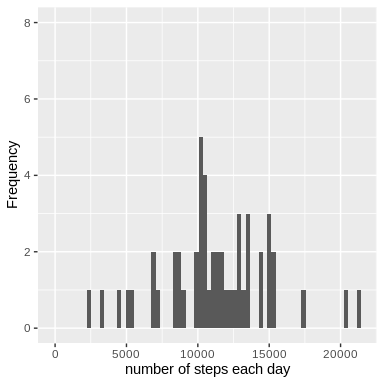
\includegraphics{PA1_template_files/figure-latex/unnamed-chunk-2-1.pdf}

\hypertarget{calculate-and-report-the-mean-and-median-total-number-of-steps-taken-per-day}{%
\subparagraph{2. Calculate and report the mean and median total number
of steps taken per
day}\label{calculate-and-report-the-mean-and-median-total-number-of-steps-taken-per-day}}

\begin{Shaded}
\begin{Highlighting}[]
\NormalTok{meanSteps }\OtherTok{\textless{}{-}} \FunctionTok{mean}\NormalTok{(stepday)}
\NormalTok{medianSteps }\OtherTok{\textless{}{-}} \FunctionTok{median}\NormalTok{(stepday)}
\end{Highlighting}
\end{Shaded}

\begin{itemize}
\tightlist
\item
  9354.2295082
\item
  10395
\end{itemize}

\hypertarget{what-is-the-average-daily-activity-pattern}{%
\subsection{What is the average daily activity
pattern?}\label{what-is-the-average-daily-activity-pattern}}

\begin{Shaded}
\begin{Highlighting}[]
\NormalTok{avgday }\OtherTok{\textless{}{-}} \FunctionTok{aggregate}\NormalTok{(data}\SpecialCharTok{$}\NormalTok{steps, }\AttributeTok{by =} \FunctionTok{list}\NormalTok{(data}\SpecialCharTok{$}\NormalTok{interval), mean, }\AttributeTok{na.rm =}\NormalTok{ T)}
\end{Highlighting}
\end{Shaded}

\hypertarget{make-a-time-series-plot-i.e.-type-l-of-the-5-minute-interval-x-axis-and-the-average-number-of-steps-taken-averaged-across-all-days-y-axis}{%
\paragraph{1. Make a time series plot (i.e.~type = ``l'') of the
5-minute interval (x-axis) and the average number of steps taken,
averaged across all days
(y-axis)}\label{make-a-time-series-plot-i.e.-type-l-of-the-5-minute-interval-x-axis-and-the-average-number-of-steps-taken-averaged-across-all-days-y-axis}}

\begin{Shaded}
\begin{Highlighting}[]
\FunctionTok{plot}\NormalTok{(avgday, }\AttributeTok{type =} \StringTok{"l"}\NormalTok{, }\AttributeTok{xlab =} \StringTok{"5{-}minute interval"}\NormalTok{, }
     \AttributeTok{ylab =} \StringTok{"Average Number of steps"}\NormalTok{, }\AttributeTok{col =} \StringTok{"dark red"}\NormalTok{)}
\end{Highlighting}
\end{Shaded}

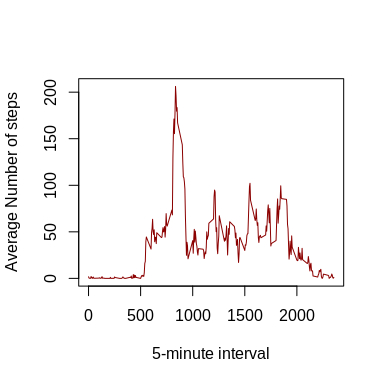
\includegraphics{PA1_template_files/figure-latex/time-1.pdf}

\hypertarget{which-5-minute-interval-on-average-across-all-the-days-in-the-dataset-contains-the-maximum-number-of-steps}{%
\paragraph{2. Which 5-minute interval, on average across all the days in
the dataset, contains the maximum number of
steps?}\label{which-5-minute-interval-on-average-across-all-the-days-in-the-dataset-contains-the-maximum-number-of-steps}}

\begin{Shaded}
\begin{Highlighting}[]
\FunctionTok{max}\NormalTok{(avgday[,}\DecValTok{1}\NormalTok{])}
\end{Highlighting}
\end{Shaded}

\begin{verbatim}
## [1] 2355
\end{verbatim}

\hypertarget{imputing-missing-values}{%
\subsection{Imputing missing values}\label{imputing-missing-values}}

\hypertarget{calculate-and-report-the-total-number-of-missing-values-in-the-dataset-i.e.-the-total-number-of-rows-with-nas}{%
\paragraph{1. Calculate and report the total number of missing values in
the dataset (i.e.~the total number of rows with
NAs)}\label{calculate-and-report-the-total-number-of-missing-values-in-the-dataset-i.e.-the-total-number-of-rows-with-nas}}

\begin{Shaded}
\begin{Highlighting}[]
\FunctionTok{length}\NormalTok{(}\FunctionTok{which}\NormalTok{(}\FunctionTok{is.na}\NormalTok{(data)))}
\end{Highlighting}
\end{Shaded}

\begin{verbatim}
## [1] 2304
\end{verbatim}

\hypertarget{devise-a-strategy-for-filling-in-all-of-the-missing-values-in-the-dataset.-the-strategy-does-not-need-to-be-sophisticated.-for-example-you-could-use-the-meanmedian-for-that-day-or-the-mean-for-that-5-minute-interval-etc.}{%
\paragraph{2. Devise a strategy for filling in all of the missing values
in the dataset. The strategy does not need to be sophisticated. For
example, you could use the mean/median for that day, or the mean for
that 5-minute interval,
etc.}\label{devise-a-strategy-for-filling-in-all-of-the-missing-values-in-the-dataset.-the-strategy-does-not-need-to-be-sophisticated.-for-example-you-could-use-the-meanmedian-for-that-day-or-the-mean-for-that-5-minute-interval-etc.}}

\begin{Shaded}
\begin{Highlighting}[]
\NormalTok{data}\SpecialCharTok{$}\NormalTok{steps }\OtherTok{\textless{}{-}} \FunctionTok{impute}\NormalTok{(data}\SpecialCharTok{$}\NormalTok{steps, mean)}
\end{Highlighting}
\end{Shaded}

\hypertarget{create-a-new-dataset-that-is-equal-to-the-original-dataset-but-with-the-missing-data-filled-in.}{%
\paragraph{3. Create a new dataset that is equal to the original dataset
but with the missing data filled
in.}\label{create-a-new-dataset-that-is-equal-to-the-original-dataset-but-with-the-missing-data-filled-in.}}

\begin{Shaded}
\begin{Highlighting}[]
\NormalTok{data}\SpecialCharTok{$}\NormalTok{steps }\OtherTok{\textless{}{-}} \FunctionTok{impute}\NormalTok{(data}\SpecialCharTok{$}\NormalTok{steps, mean)}
\end{Highlighting}
\end{Shaded}

\hypertarget{make-a-histogram-of-the-total-number-of-steps-taken-each-day-and-calculate-and-report-the-mean-and-median-total-number-of-steps-taken-per-day.}{%
\paragraph{4. Make a histogram of the total number of steps taken each
day and Calculate and report the mean and median total number of steps
taken per
day.}\label{make-a-histogram-of-the-total-number-of-steps-taken-each-day-and-calculate-and-report-the-mean-and-median-total-number-of-steps-taken-per-day.}}

\begin{Shaded}
\begin{Highlighting}[]
\NormalTok{step.imp }\OtherTok{\textless{}{-}} \FunctionTok{tapply}\NormalTok{(data}\SpecialCharTok{$}\NormalTok{steps, data}\SpecialCharTok{$}\NormalTok{date, sum)}
\FunctionTok{qplot}\NormalTok{(step.imp, }\AttributeTok{xlab =} \StringTok{"number of steps each day"}\NormalTok{, }\AttributeTok{ylab =} \StringTok{"Frequency"}\NormalTok{,}
      \AttributeTok{binwidth =} \DecValTok{300}\NormalTok{)}
\end{Highlighting}
\end{Shaded}

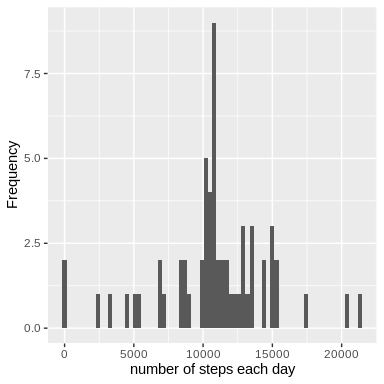
\includegraphics{PA1_template_files/figure-latex/unnamed-chunk-7-1.pdf}

\begin{Shaded}
\begin{Highlighting}[]
\NormalTok{meanSteps.imp }\OtherTok{\textless{}{-}} \FunctionTok{mean}\NormalTok{(step.imp)}
\NormalTok{medianSteps.imp }\OtherTok{\textless{}{-}} \FunctionTok{median}\NormalTok{(step.imp)}
\end{Highlighting}
\end{Shaded}

\begin{itemize}
\tightlist
\item
  \ensuremath{1.0766189\times 10^{4}}
\item
  \ensuremath{1.0766189\times 10^{4}}
\end{itemize}

Do these values differ from the estimates from the first part of the
assignment? What is the impact of imputing missing data on the estimates
of the total daily number of steps?

\hypertarget{are-there-differences-in-activity-patterns-between-weekdays-and-weekends}{%
\subsection{Are there differences in activity patterns between weekdays
and
weekends?}\label{are-there-differences-in-activity-patterns-between-weekdays-and-weekends}}

\begin{Shaded}
\begin{Highlighting}[]
\NormalTok{days }\OtherTok{\textless{}{-}} \FunctionTok{which}\NormalTok{(}\FunctionTok{weekdays}\NormalTok{(data}\SpecialCharTok{$}\NormalTok{date) }\SpecialCharTok{\%in\%}
                      \FunctionTok{c}\NormalTok{(}\StringTok{"Monday"}\NormalTok{, }\StringTok{"Tuesday"}\NormalTok{, }\StringTok{"Wednesday"}\NormalTok{, }\StringTok{"Thursday"}\NormalTok{, }\StringTok{"Friday"}\NormalTok{))}
\NormalTok{end }\OtherTok{\textless{}{-}} \FunctionTok{which}\NormalTok{(}\FunctionTok{weekdays}\NormalTok{(data}\SpecialCharTok{$}\NormalTok{date) }\SpecialCharTok{\%in\%}
                     \FunctionTok{c}\NormalTok{(}\StringTok{"Saturday"}\NormalTok{, }\StringTok{"Sunday"}\NormalTok{))}

\NormalTok{data[end,}\DecValTok{4}\NormalTok{] }\OtherTok{\textless{}{-}} \StringTok{"weekend"} 
\NormalTok{data[days,}\DecValTok{4}\NormalTok{] }\OtherTok{\textless{}{-}} \StringTok{"weekday"}
\end{Highlighting}
\end{Shaded}

\hypertarget{create-a-new-factor-variable-in-the-dataset-with-two-levels-weekday-and-weekend-indicating-whether-a-given-date-is-a-weekday-or-weekend-day.}{%
\paragraph{1. Create a new factor variable in the dataset with two
levels -- ``weekday'' and ``weekend'' indicating whether a given date is
a weekday or weekend
day.}\label{create-a-new-factor-variable-in-the-dataset-with-two-levels-weekday-and-weekend-indicating-whether-a-given-date-is-a-weekday-or-weekend-day.}}

\begin{Shaded}
\begin{Highlighting}[]
\NormalTok{data[,}\DecValTok{4}\NormalTok{] }\OtherTok{\textless{}{-}} \FunctionTok{as.factor}\NormalTok{(data[,}\DecValTok{4}\NormalTok{])}
\FunctionTok{colnames}\NormalTok{(data) }\OtherTok{\textless{}{-}} \FunctionTok{c}\NormalTok{(}\StringTok{"steps"}\NormalTok{, }\StringTok{"date"}\NormalTok{, }\StringTok{"interval"}\NormalTok{, }\StringTok{"week"}\NormalTok{)}
\end{Highlighting}
\end{Shaded}

\hypertarget{make-a-panel-plot-containing-a-time-series-plot-i.e.-type-l-of-the-5-minute-interval-x-axis-and-the-average-number-of-steps-taken-averaged-across-all-weekday-days-or-weekend-days-y-axis}{%
\paragraph{2. Make a panel plot containing a time series plot (i.e.~type
= ``l'') of the 5-minute interval (x-axis) and the average number of
steps taken, averaged across all weekday days or weekend days
(y-axis)}\label{make-a-panel-plot-containing-a-time-series-plot-i.e.-type-l-of-the-5-minute-interval-x-axis-and-the-average-number-of-steps-taken-averaged-across-all-weekday-days-or-weekend-days-y-axis}}

`

\begin{Shaded}
\begin{Highlighting}[]
\NormalTok{avgday.imp }\OtherTok{\textless{}{-}} \FunctionTok{aggregate}\NormalTok{(steps }\SpecialCharTok{\textasciitilde{}}\NormalTok{ interval }\SpecialCharTok{+}\NormalTok{ week, mean, }\AttributeTok{data =}\NormalTok{ data)}


\FunctionTok{xyplot}\NormalTok{(}\FunctionTok{log10}\NormalTok{(steps) }\SpecialCharTok{\textasciitilde{}}\NormalTok{ interval }\SpecialCharTok{|}\NormalTok{ week, }\AttributeTok{data =}\NormalTok{ data,}\AttributeTok{layout=}\FunctionTok{c}\NormalTok{(}\DecValTok{1}\NormalTok{,}\DecValTok{2}\NormalTok{),}
       \AttributeTok{type =} \StringTok{"l"}\NormalTok{, }\AttributeTok{strip =}\NormalTok{ T, }\AttributeTok{xlab =} \StringTok{"5{-}minute interval"}\NormalTok{,}
       \AttributeTok{ylab =} \StringTok{"Average of weekdays/weekend"}\NormalTok{)}
\end{Highlighting}
\end{Shaded}

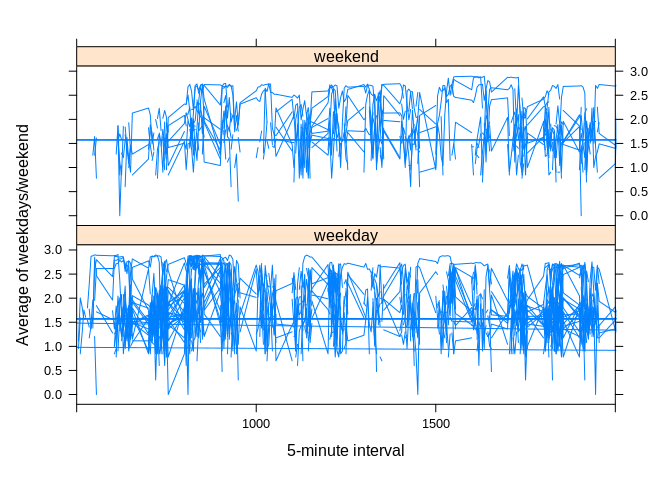
\includegraphics{PA1_template_files/figure-latex/unnamed-chunk-11-1.pdf}

\end{document}
